\documentclass{article}
\usepackage{amsmath}
\usepackage{enumitem}
\usepackage{amssymb}
\usepackage{tikz}
\usepackage{bbm}
\usepackage{geometry}
\usepackage{mathtools}
\usepackage{amsthm}
\usepackage{graphicx}
\DeclareMathOperator*{\argmin}{arg\!\min}
\DeclareMathOperator*{\argmax}{arg\!\max}

\geometry{letterpaper, portrait, margin=1in}
\newcommand{\ul}[0]{\underline}
\newcommand{\hs}[1]{\hspace*{#1 cm}}
\newcommand{\ind}[0]{\indent}
\newcommand{\tx}[1]{\text{#1}}

\newtheorem{theorem}{Theorem}[section]
\newtheorem{corollary}{Corollary}[theorem]
\newtheorem{lemma}[theorem]{Lemma}
\newtheorem{remark}{Remark}


\title{Genre Classification of YouTube Videos}
\author{
  Modzelewski, Derek\\
  \texttt{dmodzel2@jhu.edu}
  \and
  Smillie, Dan\\
  \texttt{dsmilli1@jhu.edu}
}

\begin{document}

\maketitle

\tableofcontents

\section{Overview} %Dan

\ind\ind YouTube has a massive collection of videos, and many of them are labeled for search visibility. This dataset is a huge opportunity to do video classification. To facilitate this, Google has (very very recently) released tools to reduce the size of the data and make it accessible to researchers without hundreds of CPU years at their disposal.

We use this data to train a classifier to label videos, demonstrate that some labels are harder to learn than others, and show the model’s efficacy on wild videos. \\
\\
Our work is on Github at: \textcolor{blue}{https://github.com/Derekmod/CV\_final.git}


\section{Dataset} %Dan

\ind\ind The Youtube-8M dataset is a large-scale labeled video dataset that is compromised of millions YouTube video ID’s and labels from over 4700 classes of labels. The data is precomputed so as to reduce the size from {\it hundreds} of Terabytes of data, to merely Gigabytes. This dataset is especially exciting to be working with because of how recently it has been released to the public. Google and YouTube first announced the dataset in September of 2016 and has even released new feature extraction code in November of this year, which we were able to work with. 

The dataset comes in two major flavors, video level and frame level features. Despite the fact that over seven million videos have been used to build this set, the fully compressed dataset is still smaller than two terabytes. 

The labels, that are coupled with the video ID’s, represent different categories of video. For example a video of Lebron James dunking in the middle of a basketball game would receive the labels, sports, game, and possibly celebrity. The average number of labels per video is about three and a half. 

The dataset also contained audio features that we did not manipulate in any way but we hypothesized about how coupling those features along with frame and/or video level features could lead to interesting results.


\section{Methods} %Derek

\subsection{Models}

\ind\ind Google has published support for training Logistic multi-class classifiers for both frame-level and video-level features. Although this is a simple model, we expect it to be sufficient since the data is already preprocessed in a (hopefully) intelligent manner. It would be interesting to see if a shallow neural-network would perform better, but we didn't have the time to reverse-engineer Google's code and create our own model.

Since both frame-level and video-level features have the same (well-studied) model, any differences in the results should reflect the differences in aptitudes of the features, not the models.

\subsection{Training}

\ind\ind We used over a million videos and 3000 steps for both frame-level and video-level features. We saw that the learning rate for both types of features are nearly identical.

\subsection{Evaluation}

\ind\ind When we started this project, one of the core things we wanted to show was the difference in ability to learn different labels. This is not built into Google’s simple package, so we had to make it ourselves. We used Binary Cross Entropy Loss to evaluate the outputted label probabilities, setting the predicted probability to $0.5\%$ as it seems TensorFlow does not report labels with less than $1\%$ probability.

Using this data, we can generate plots for each label of error vs. iteration, and possibly plot the errors of two labels against each other vs. iteration. The hope of this method is to highlight whether or not some labels train better than other labels. However, Google has some hidden bugs in their code and many of our label error files are basically useless.

\section{Results}

\subsection{Total Error by Iteration}
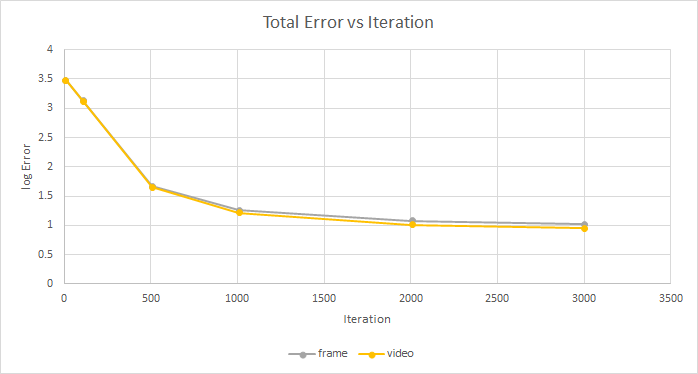
\includegraphics[scale=1.8]{Error_vs_Step.png} \\
Above shows {\it validation} error, and so reflects the generalizability of the models, not just the training accuracy. We see that the two models start with the same error, but {\it slowly} diverge {\it s.t.} video features are slightly superior.
\\
\\
Contrarily, for training error, the model using frame-features outperformed the video-features one with a score of $8.5$ whereas video-features had a score of $35$ \\

\subsection{Compare Label Error}
See "err\_3000.xlxs" for results. \\\\
\ind\ind We were able to evaluate the individual label errors at the final iteration. While we are not confident the code ran $100\%$ correctly, there are some patterns in the results which are worth mentioning:
\begin{enumerate}
\item Errors are higher for more common labels. \\
\ind\ind This is because the frequencies are closer to $50\%$ for more common labels, making a naive predictor (simply predict the training frequency as probability) less successful. Thus, it is harder to achieve the same error rate.
\item Some labels are relatively hard to classify:
	\begin{enumerate}
	\item Motorsport
	\item Cartoon
	\item Performance Art
	\item Mobile Phone
	\item Smartphone
	\item Motorcycle
	\end{enumerate}
\item Some labels are relatively easy to classify:
	\begin{enumerate}
	\item Nature
	\item String Instrument
	\item Fashion
	\item Art
	\end{enumerate}
\end{enumerate}

\subsection{Label Error by Iteration}
Too many bugs to have meaningful results.

\subsection{Improvement in Prediction}
See "predictions50.csv" and "predictions3000.csv" for results. \\
\\
\ind As mentioned earlier, Google has published the ability to extract the frame-features from ANY video. We got the frame-features for a Twitch Fails video, which is related to PC games. When we used a young model (after 50 iterations) to predict the labels, we found that it suggested a $40\%$ probability to every class, which neither discriminates correctly against classes nor correctly predicts the total number of classes associated.

When we used an older model (after 3000 iterations), we found that the predictions made much more sense. It was most sure that the video was related to Games, Video Games, and PC Games - exactly as we would hope.

\section{Conclusions}

\subsection{Video-Level Features Generalize Best}
\ind\ind As we see in the plot of validation error vs. iteration, video-features get more and more superior to frame-features as training time increases. Furthermore, it seems that This means that it more accurately captures the true structure of the labeling problem. In short, the results suggest that video-features are more informative than frame-freatures.

However, neither model reached convergence so it is not proven that video-features are superior. We are only fairly certain in our conclusion, not absolutely certain.

\subsection{Not All Labels are Equal}
\ind\ind We showed that some labels are easier to learn than others (even beyond the difficulties from differing frequencies). As a general pattern, we see that most of the difficult labels require object recognition of some sort. E.g. It is necessary to be able to recognize a motorcycle when distinguishing a motorcycle video from a car video. Since the YouTube-8M dataset does not save pixel data (only frame-level features such as mean-rgb values), it is impossible to perform such a recognition task and so those labels are just extremely difficult. On the other hand, the easy labels seem to have more consistent themes. Nature videos are presumably very green, and art videos probably have one object in the middle and very little fast movement in the video. 

Everything indicates that our model is atune to these consistent features and successful at reporting which labels are hardest to predict. This technology might be used in CCTV to give reasoning to why some types of behavior are harder to catch than others.

\subsection{Created a Productive Model for Classifying Any Video}
We showed that we can take a Twitch video and correctly classify it, so we conclude that we could also take any other video that is represented in the training data and classify it well. For instance, we would do well at identifying fashion shows (fashion was one of the labels we found was easy to classify as well).


\section{References}

YouTube-8M: \textcolor{blue}{https://research.google.com/youtube8m/index.html}






%

\end{document}